\chapter{Il percorso di stage }\label{cap:Il_percorso}
\section{Formazione}
Il processo di formazione che mi è stato fornito ha avuto un ruolo fondamentale nella buona riuscita del progetto di stage, 
ha avuto una durata di circa 4 settimane. \\
La causa del protrarsi del processo di formazione è stata provocata dal fatto che concetti legati all'architettura \gls{eda}{},
\textbf{Apache Kafka}, \textbf{Apache Druid}, \textbf{Docker Compose} sono state del tutto innovative per me.\\
Tutto il processo di formazione è stato tracciato e monitorato dal tutor aziendale e da me stesso attraverso le \gls{board}{} offerte 
dal software di project management \textbf{ClickUp} (Figura \ref{cap:ClickUp}).\\
\begin{figure}[h]
    \centering
    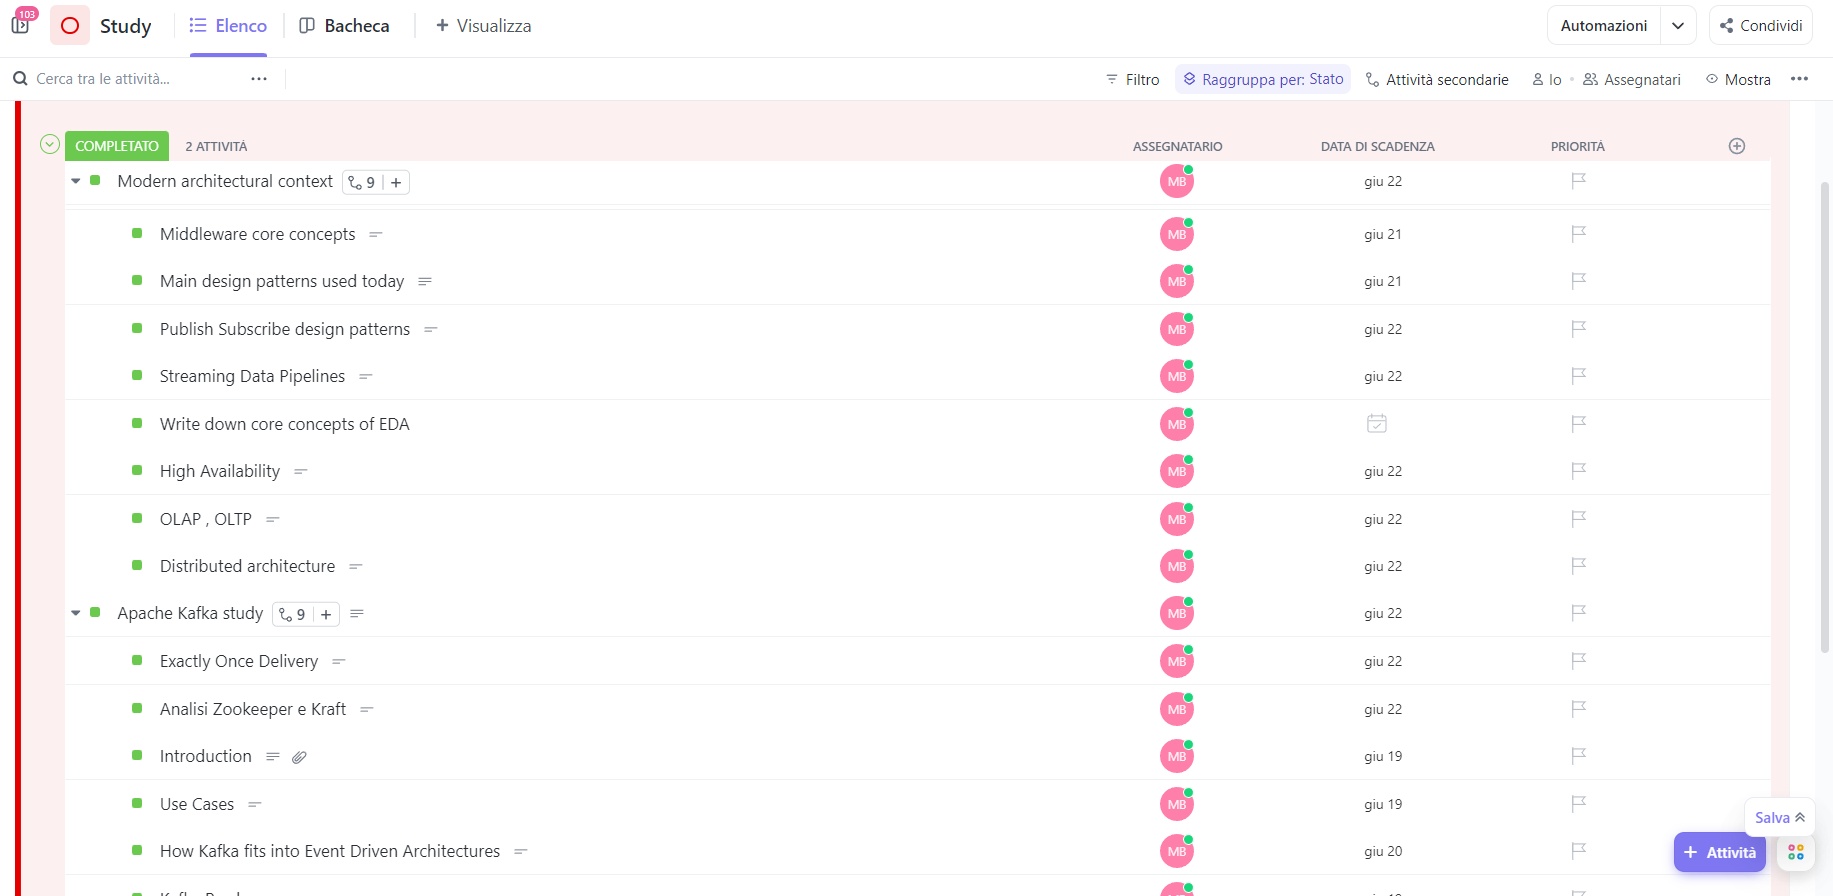
\includegraphics[width=1\textwidth]{images/percorso/formazione.png}
    \caption{Board di ClickUp per il processo di formazione}
    \label{cap:ClickUp}
\end{figure}
\pagebreak
\\
Inoltre durante il processo di formazione, oltre a reperire informazioni da documentazione ufficiale fornita , ho avuto anche modo 
di approfondire quanto appena appreso attraverso delle attività di \gls{hands-on}{} che mi hanno permesso di mettere in pratica quanto appreso (Figura \ref{cap:Hands-on}).
\begin{figure}[h]
    \centering
    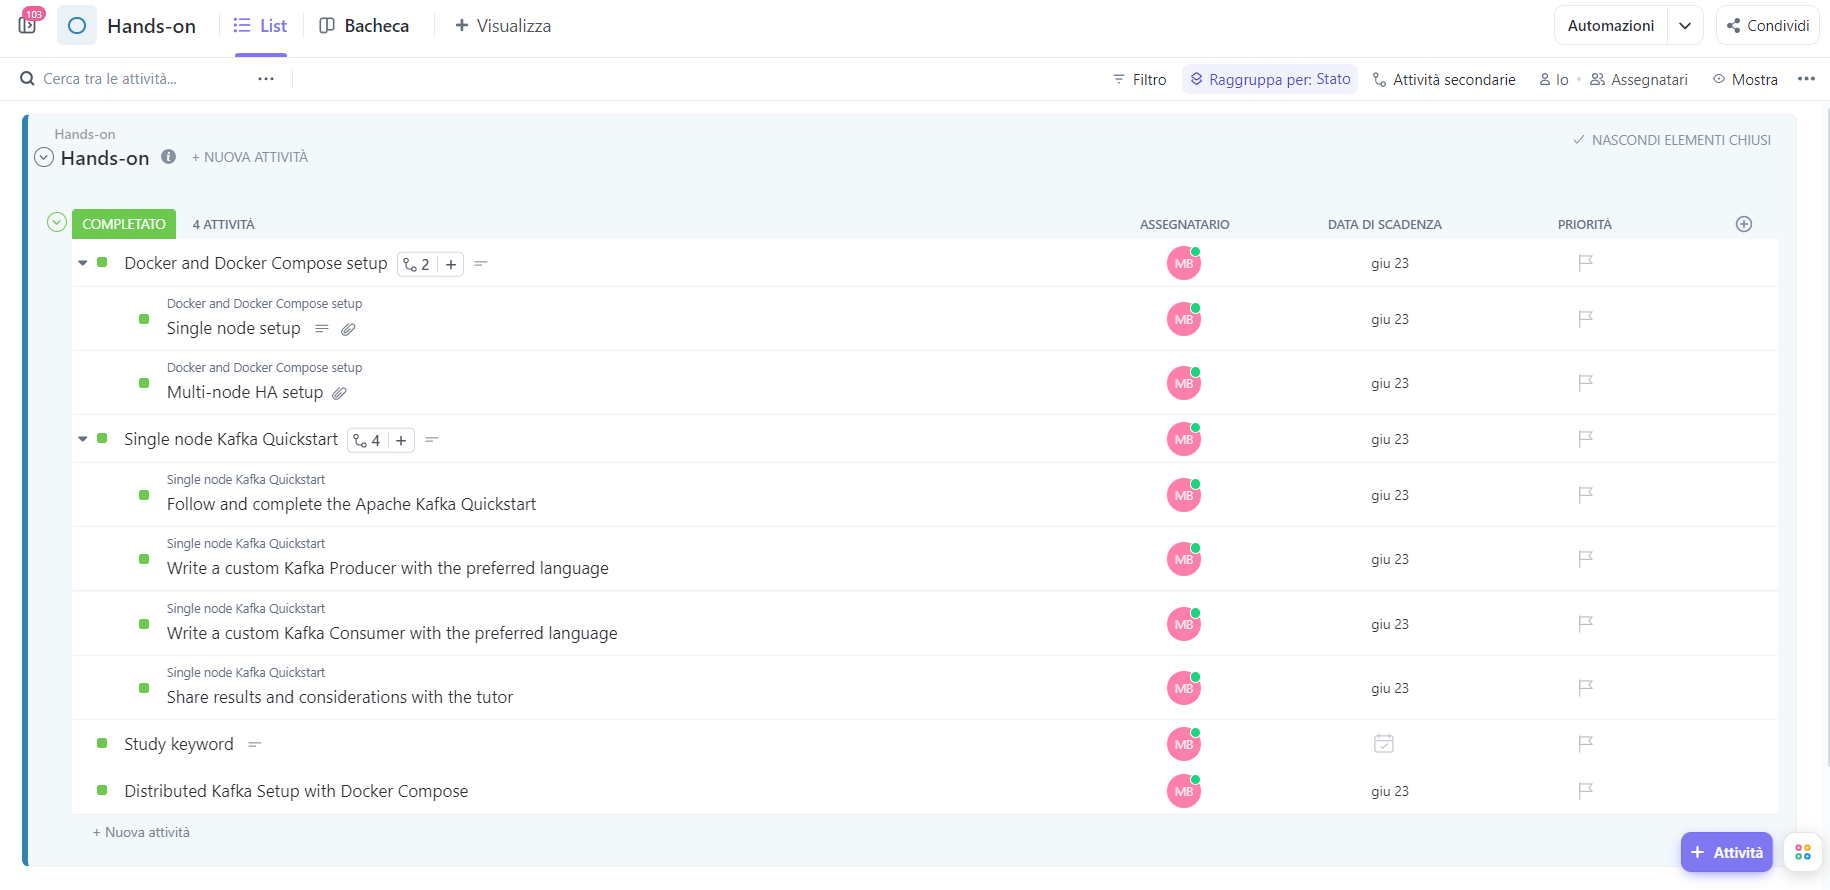
\includegraphics[width=1\textwidth]{images/percorso/hands_on.png}
    \caption{Attività di hands-on per il processo di formazione}
    \label{cap:Hands-on}
\end{figure}
\\
Oltre a ciò, durante il processo di formazione, in collaborazione con il tutor aziendale, è stato definito un processo di coordinamento e produzione di 
documentazione tecnica che mi ha permesso durante tutto lo svolgimento del percorso di stage di avere un tracciamento dei concetti appresi 
e di avere riferimenti per la risoluzione di problemi o dubbi sorti (Figura \ref{cap:Documentazione})
\begin{figure}[h]
    \centering
    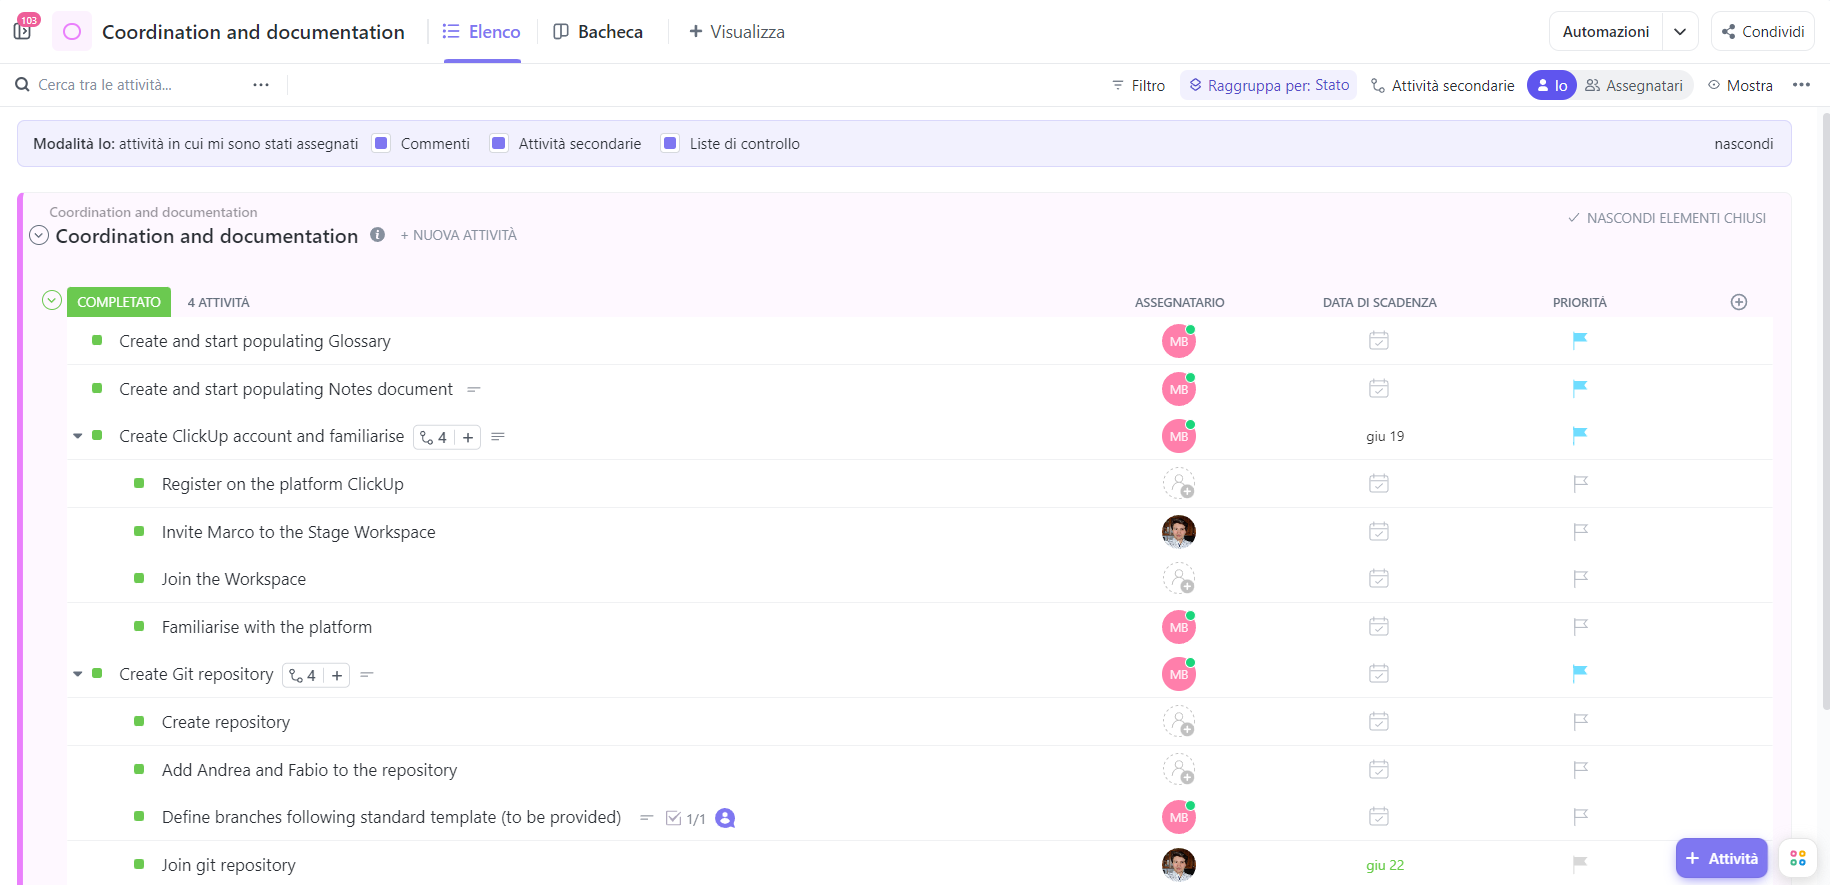
\includegraphics[width=1\textwidth]{images/percorso/coordinamento.png}
    \caption{Board di ClickUp per il processo di coordinamento e documentazione}
    \label{cap:Documentazione}
\end{figure}
\newpage
\pagestyle{empty}
\null % o \mbox{} o \phantom{X}
\newpage